
%body poses $\{\bm{\theta}^{(t)}\}$, node residual translations $\{\Delta\bm{n}_i^{(t)}\}$ and dynamic detail embeddings $\{\bm{e}_i^{(t)}}\}$.

\section{Method}
\label{sec:method}
Having elaborated on the proposed representation, we turn to network learning in this section. 
Specifically, we need to determine the aforementioned variables alongside with the weights of the radiance networks for a training image sequence $\bm{I}_t, t=1, 2,..., T$. The images can be captured from a multi-view system or a monocular one. In order to synthesize images for new poses, we also have to compute the node residual translations and the dynamic detail embeddings corresponding to those poses. 
We assume access to the body poses of the training images (\textit{i.e.}, $\bm{\theta}^{(t)}, t=1, 2, ..., T$), which can be estimated using marker-less MoCap tools such as \cite{easymocap,lightcap2021}. The node residual translations and the detail embeddings are referred to as ``node-related variables" in the following context. 



% Having elaborated on the proposed representation, we turn to network learning in this section. 
% Specifically, we need to determine the aforementioned variables (i.e., body poses, node residual translation and dynamic detail embeddings) as well as the weights of the radiance networks for a training sequence $\bm{I}_t, t=1, 2,..., T$. In order to synthesize images for new poses, we also have to compute the node residual translations and the dynamic detail embeddings corresponding to those specific poses. In this work, we assume access to the body poses of the training images, which can be easily obtained using existing marker-less MoCap algorithm such as \cite{easymocap}. 

% In Sec.~\ref{sec:method:arch} and ~\ref{sec:method:loss}, we discuss how to determine the aforementioned variables as well as the weights of the radiance networks for a training image sequence $\bm{I}_t, t=1, 2,..., T$. In order to synthesize images for new poses after training, we also need to compute the node residual translations and the dynamic detail embeddings corresponding to those specific poses (Sec.~\ref{sec:method:animation}). In this work, we assume access to the body poses of the training images, which can be easily obtained using existing marker-less MoCap algorithm such as \cite{easymocap}. 


\subsection{Network Architecture}
\label{sec:method:arch}
To obtain the node-related variables for the training frames and ensure generalization during animation, we design a simple conditional variational auto-encoders (cVAE)~\cite{Sohn2015cvae} as an auxiliary network for each node. 
% Naive optimization during network training make it difficult to generate the variables for new poses after training, while directly regressing them from pose condition leads to one-to-many problem as the similar poses can lead to different cloth wrinkles in reality. 
% A naive solution to obtain the node residual translation and dynamic detail embeddings is using optimization during network training (i.e., auto-decoding~\cite{park2019deepsdf}). However, this will make it difficult to generate the variables for new poses during training. What's worse, naive optimization cannot guarantee information distanglement, which further hinders generalization~\cite{timur2021driving_signal}. 
% Drawing inspiration from \cite{timur2021driving_signal}, we design a simple conditional variational auto-encoder ~\cite{Sohn2015cvae} for each node as an auxiliary network. Each cVAE consists of an encoder and a decoder, both implemented with MLPs. 
Each auxiliary network consists of an encoder and a decoder, both implemented with tiny MLPs. 
Following the practice of SCANimate~\cite{Saito:SCANimate:2021}, the condition variable of this cVAE is the pose vector multiplied by the skinning weight and an attention map:
\begin{equation}
    \bm{\theta}^{(t)}_i = (\bm{\mathrm{W}}\cdot \bm{\omega}_i) \circ \bm{\theta}^{(t)}, 
\end{equation}
where $\bm{\mathrm{W}}$ is the weight map that converts the skinning weights into pose attention weights as in \cite{Saito:SCANimate:2021} and $\circ$ denotes element-wise product. 
During training, the encoder takes the time stamp $t$ as input and $\bm{\theta}^{(t)}_i$ as condition, and produces parameters of a Gaussian distribution, from which a latent code $\bm{z}_i^{(t)}$ is sampled:
\begin{equation}
\label{eqn:latent_sample}
    \bm{\mu}_i^{(t)}, \bm{\sigma}_i^{(t)} \gets \mathcal{E}(t, \bm{\theta}_i^{(t)}), \ \bm{z}_i^{(t)} \sim \mathcal{N}(\bm{\mu}_i^{(t)}, \bm{\sigma}_i^{(t)}), 
\end{equation}
% In practice we augment the time stamp with periodic encoding~\cite{mildenhall2020nerf}. 
Conditioned on the body pose, the latent code is then decoded into the node residual translation and the dynamic detail embedding:
\begin{equation}
    \Delta\bm{n}_i^{(t)},  \bm{e}_i^{(t)} \gets \mathcal{D}(\bm{z}_i^{(t)}, \bm{\theta}_i^{(t)}), 
\end{equation}
which are later used in Eqn.~(\ref{eqn:reprez:local_coord}) and  Eqn.~(\ref{eqn:reprez:feat_fusion}), respectively. 

In this network, the time instant is used to distinguish similar poses at different time instants, thereby avoiding the one-to-many mapping issue. With the KL-divergence loss in cVAE, there is a preference to let the decoder to mainly rely on the pose condition for prediction, and the time input only provides information necessary for good reconstruction.  
In our implementation, we augment the time stamp and the coordinates with Fourier encoding before feeding them into MLPs~\cite{mildenhall2020nerf} . Fig.~\ref{fig:network} illustrates the data flow in our network during training. Once the training is done, we can render the model for either training frames or novel poses. To render the training sequence, we use the full network and set $\bm{z}_i^{(t)} = \bm{\mu}_i^{(t)}$ in Eqn.~(\ref{eqn:latent_sample}) to eliminate randomness. When unseen poses are given, the encoder half of the cVAE will be omitted and $\bm{z}_i^{(t)}$ will be set to zeros. 


\subsection{Training Loss}
\label{sec:method:loss}
Our network can be trained in an end-to-end manner. 
The training loss is composed of four components, including a reconstruction loss, a node translation regularization, an embedding regularization, and a KL-divergence loss:
\begin{equation}
     \mathcal{L} = \lambda_{rec}\mathcal{L}_{rec} + \lambda_{trans}\mathcal{L}_{trans} + \lambda_{ebd}\mathcal{L}_{ebd} + \lambda_{KL}\mathcal{L}_{KL}.
\end{equation}
Below we discuss them in details. For ease of notation, we drop the superscript ${}^{(t)}$ of all variables in this subsection. 

\textbf{Reconstruction Loss} $\mathcal{L}_{rec}$ measures the mean squared error between the rendered and true pixel colors:
\begin{equation}
    \mathcal{L}_{rec} = \sum_{\bm{r}\in\mathcal{R}} \left\Vert \bm{C}\left(\bm{r} | \bm{\theta}, \{\Delta\bm{n}_i\}, \{\bm{e}_i\}\right) - \hat{\bm{C}}_{\bm{r}}  \right\Vert_2^2, 
\end{equation}
where $\mathcal{R}$ is the set of rays in each batch, $\hat{\bm{C}}_{\bm{r}}$ is the ground-truth pixel color, $\bm{C}(\cdot | \bm{\theta}, \{\Delta\bm{n}_i\}, \{\bm{e}_i\})$ is the volume rendering function with the representation defined in Sec.~\ref{sec:overview}. 

\textbf{Node Translation Regularization} $\mathcal{L}_{trans}$ simply constrains the position change of each nodes in order to stabilize training: 
\begin{equation}
    \mathcal{L}_{trans} = \sum_i \Vert \Delta\bm{n}_i \Vert_2^2. 
\end{equation}

\textbf{Embedding Regularization} $\mathcal{L}_{ebd}$ penalize large magnitudes of the dynamic detail embeddings: 
\begin{equation}
    \mathcal{L}_{ebd} = \sum_i \Vert \bm{e}_i \Vert_2^2. 
\end{equation}
% It is inspired by \cite{park2019deepsdf} and 
A similar loss is also used in \cite{park2019deepsdf}; here we utilize it to encourage the embeddings to encode only the information that cannot be represented by node position. 
%and can push the latent embeddings to become uninformative. 
% Through tuning the value of $\lambda_{trans}$ and $\lambda_{ebd}$, we can encourage the embeddings to encode only the information that cannot be represented by node position. 

\textbf{KL-divergence Loss} $\mathcal{L}_{KL}$ is a standard VAE KL-divergence penalty~\cite{kingma2014vae}:
\begin{equation}
    \mathcal{L}_{KL} = \sum_i \mathrm{KL}\left( \mathcal{N}(\bm{\mu}_i, \bm{\sigma}_i) \ \Vert\  \mathcal{N}(\bm{0}, \bm{\mathrm{I}})\right).
\end{equation}

% \subsection{New Pose Synthesis}
% \label{sec:method:animation}


\begin{figure}
    \centering
    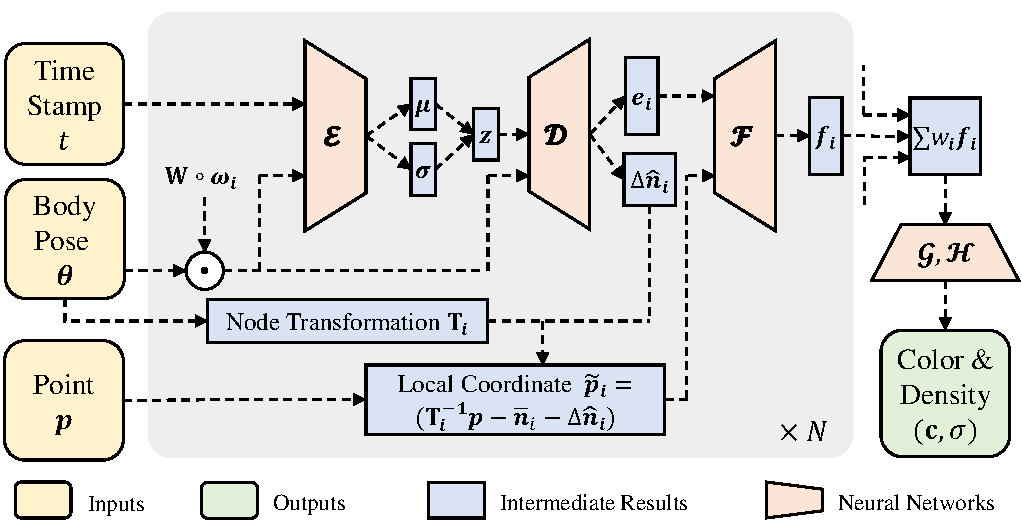
\includegraphics[width=1.0\linewidth]{network}
    \caption{\textbf{Illustration of the data flow in our network.} The time stamp and body pose feature are first passed through the cVAEs, which produces the node residual translations and dynamic detail embeddings of the local radiance fields. For a point in the posed space, we calculate its local coordinate in each local field, and then query its feature. Finally, all features are blended and decoded into the color and density values.   }
    \label{fig:network}
\end{figure}





\noindent\textbf{Implementation Details}
The local radiance networks and cVAEs in our architecture are implemented with parallel tiny MLPs in the form of group 1D convolution.
To accelerate training and inference, we exploit the fact that, for any point in the posed space, only a small portion of nodes have influence on its color and density value. 
We use Adam optimizer to train our models. Training the whole models takes about 25 hours on one NVIDIA 3090 GPU with 500k iterations, while rendering an color image with resolution of $512\times 512$ typically takes 5 seconds on one NVIDIA 3080TI GPU. Please refer to the \textit{Supp.Mat.} for more details. 
